\section{De la notation musicale}
Comme le dit Jean-Yves Bosseur dans \cite{bosseur2005}, l'évolution perpétuelle de la notation musicale au fil du temps témoigne du caractère versatile de la pensée compositionnelle, qui est fonction de trois entités : le compositeur, l'interprète et le cadre socio-technologique d'une époque.
A travers l'histoire, la présente partie veut suggérer au lecteur la difficulté de l'écriture musicale, et la nécessité de sa réinvention constante.
Pour plus de clarté, l'histoire de la notation musicale est découpée en périodes historiques ne rendant pas entièrement compte du caractère continuel de l'évolution de la Musique.   


\paragraph{Antiquité et Moyen-Age} Le premier exemple d'une notation musicale apparaît au IIIe siècle av. J-C en Grèce avec la notation \textit{boécienne}. A cette époque, les notes de la gamme sont représentées par des lettres de l'alphabet.
Cette représentation est conçue dans une acception théorique pure visant à modéliser la relation entre les sons musicaux et les matières scientifiques, notamment les mathématiques.

Au IXe siècle, plusieurs exemples de parchemins retranscrivant des chants liturgiques sont annotés par des symboles appelés \glspl{neume}.


\begin{figure}[!htbp]
	\centering
	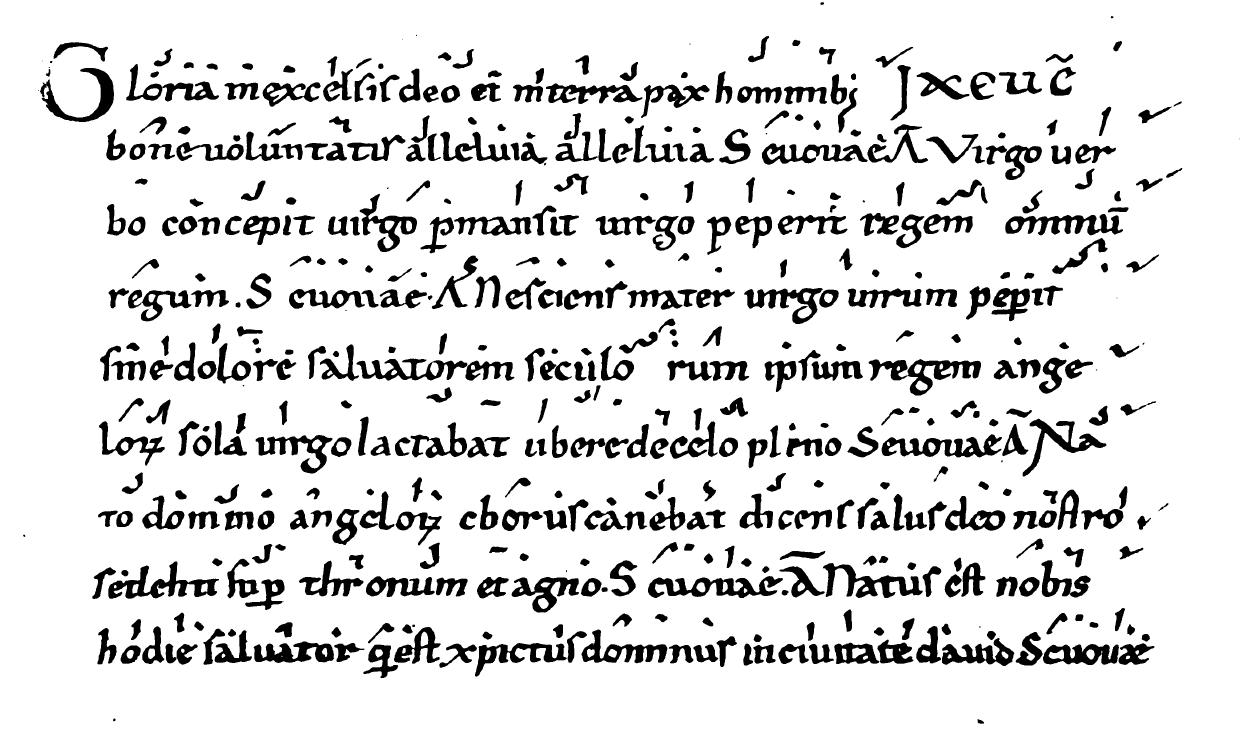
\includegraphics[keepaspectratio=true, width=0.6\textwidth]{Notation/i/neumes.jpg}
	\caption{Exemple de texte neumé - Source : 1774, Martin Gerbert, \textit{De cantu et musica sacra a prima Ecclesiae aetate usque ad praesens Tempus}, St. Blasien, Typis San-Blasianis, t. I, t. II. - \textit{Les neumes sont les symboles inscrient au-dessus des mots du chant liturgique (ici le chant} Gloria \textit{de l'ordinaire de la messe).} }
	\label{fig:neumes}
\end{figure}

Ces symboles, dont des exemples sont présentés en figure \ref{fig:neumes}, ont pour de but de décrire approximativement les inflexions mélodiques de la voix. Par exemple, le neume "point" (\textit{punctum}) indique le chant d'une note isolée; le neume "virgule" (\textit{virga}), représenté par un accent aigu, indique le chant à un intervalle supérieur vis à vis d'un neume "point".

Déjà, la notation neumatique témoigne de la volonté de fixation des caractéristiques du son chanté par le symbole. Ici, la dimension fixée est la hauteur relative des sons entre eux.

Cependant, la notation neumatique n'est pas unifiée, de telle manière que la forme des symboles disposés au-dessus du texte liturgique varie selon les régions, et même selon les moines copistes qui apposent les signes.

En effet, l'utilisation par certains clercs de la plume d'oie conduit peu à peu à l'adoption de la notation "carrée" vers la fin du XIIème siècle (voir figure \ref{fig:notationCarree}). L'embout de la plume d'oie étant bizauté, le tracé de forme carré était rendu plus facile pour le copiste.

La notation carrée (1175-1225), suivie par la notation noire (1250-1450), factorisent la profusion symbolique des neumes et coïncident avec la volonté de noter les pièces polyphoniques qui font leurs apparitions entre le Xème et XIème siècle.

La \gls{polyphonie}\footnote{Combinaison de plusieurs voix ou parties mélodiques, dans une composition musicale.} cristallise l'intérêt des compositeurs pour les relations de durée entre les différentes voix; petit à petit une notation rythmique va voir le jour.

Entre le XIIIème et le XIVème siècle, les notes se voient d'abord associées une durée relative aux modes rythmiques de chant. Les modes rythmiques quantifient le temps par un ordonnancement de notes longues et brèves.

De fait, c'est à cette époque que la barre verticale représentant la mesure fait son apparition sur la portée. La mesure regroupe, en ce temps, les ensembles de notes selon le mode rythmique employé dans la pièce musicale.

Dans la continuité de cette période, les symboles de notes se multiplieront et mèneront à une fixation absolue des valeurs rythmiques (c'est à dire, à un symbole est associé une durée).

\begin{figure}[H]
	\centering
	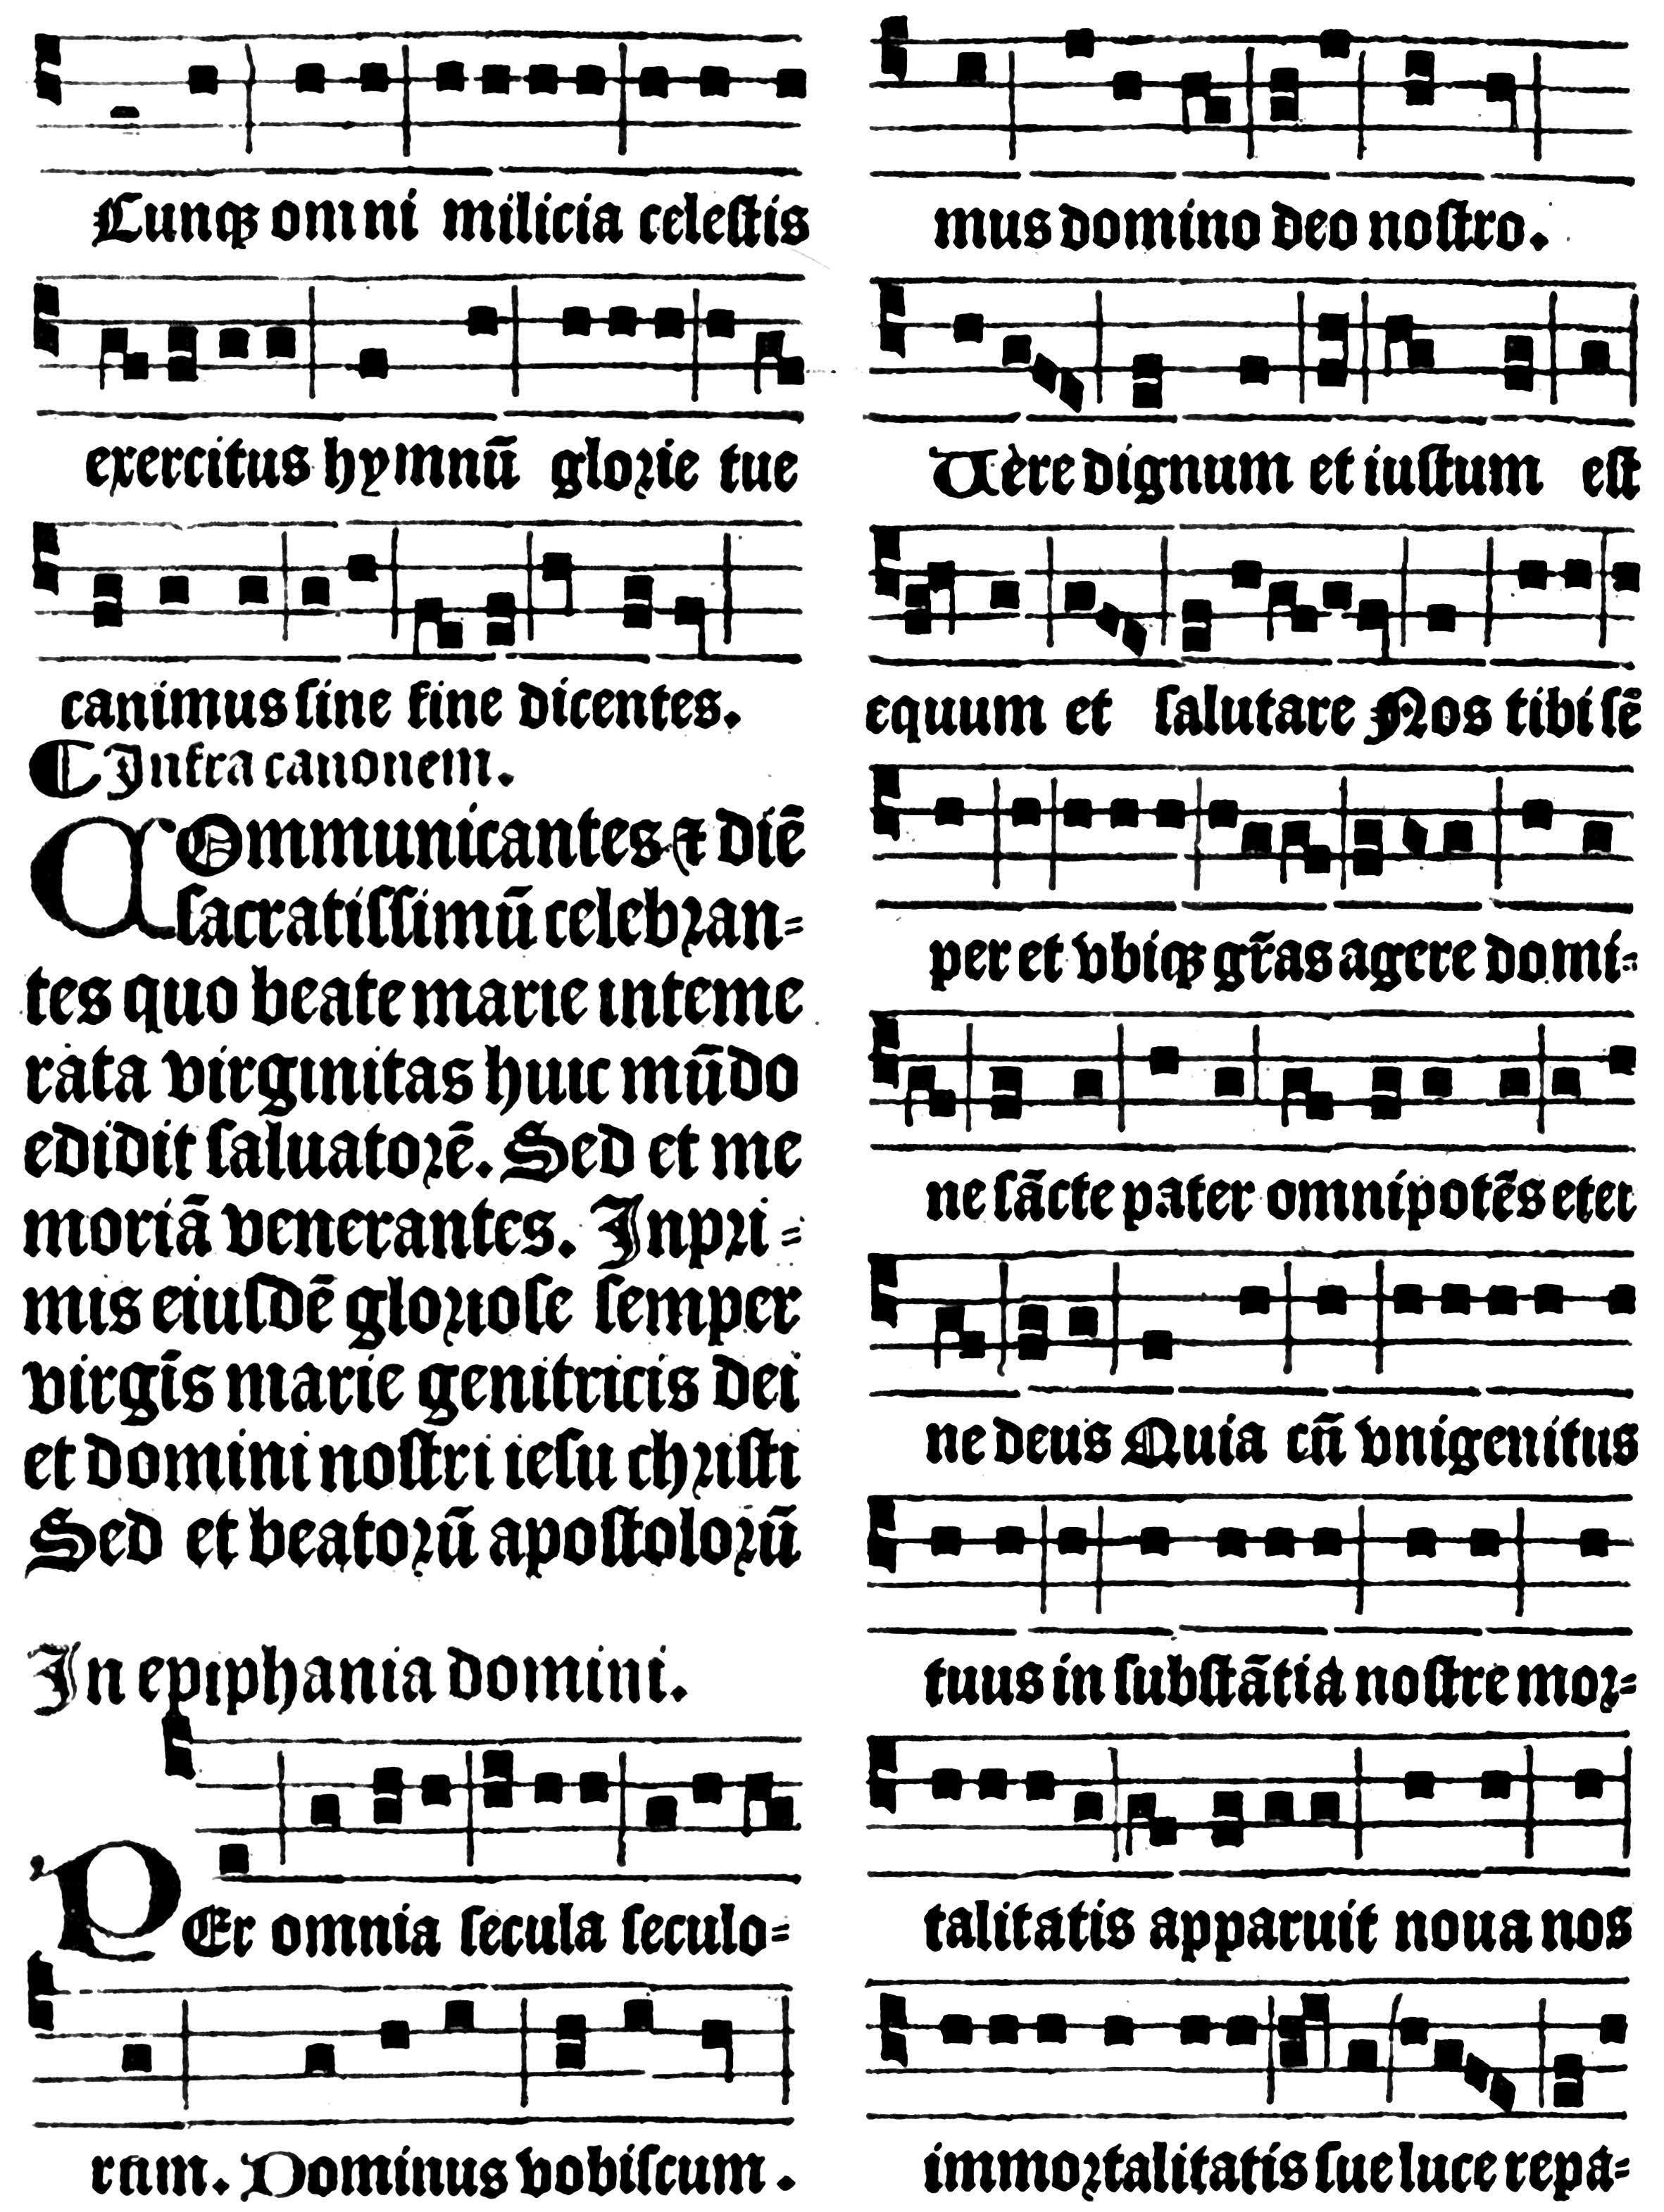
\includegraphics[keepaspectratio=true, width=0.5\textwidth]{Notation/i/notationCarree.jpg}
	\caption{Exemple de notation carrée "imprimée" - Source : 1499, Jean Highman, \textit{Missale Leodiense}, Paris - \textit{Les notes sont représentées en notation carrée toujours au-dessus du texte chanté.} }
	\label{fig:notationCarree}
\end{figure}
\todo[inline]{Trouver une autre image plus petite pour illustrée la notation carrée}

Au XIIIème siècle, une \gls{portee} stable (quatre barres pour la liturgie, cinq barres pour les autres chants) fait son apparition; portée qui jusqu'à présent restait à l'état de simple trait, dessiné discrètement par le moine copiste comme aide pour le placement des notes. Ainsi, la hauteur des notes devient fixée strictement, notamment par l'apposition de clés (clé de Fa, de Ut et de Sol) au début de la partition.

Il est a noté que l'apparition des noms des notes de la gamme date du XIème siècle environ. Les noms correspondent au premières lettres d'un hymne à Saint Jean-Baptiste :

\begin{center}
	\textbf{UT} queant laxis - \textbf{RE}sonare fibris - \textbf{MI}ragestorum - \textbf{FA}muli tuorum -  \textbf{SOL}ve pollueti - \textbf{LA}billi reatum - \textbf{S}ancte \textbf{I}ohannes
\end{center}

La fin du XIVème siècle voit poindre "une phase de complication et d'intrications inégalées"\cite{bosseur2005} en termes de notation musicale. Vient s'ajouter à la variété des symboles musicaux un système de couleur qui adjoint une sémantique rythmique supplémentaire aux pièces musicales.

A cette époque, la partition perd sa fonctionnalité de transmettrice d'informations pour l'exécution musicale d'une pièce. Cette période correspond à l'âge d'or des moines-copistes, ce qui explique l'émulation notationnelle qui fait ressembler les partitions à de véritables oeuvres graphiques, délaissant la compréhension des pièces par les interprètes.

Comme le fait remarquer Jean-Yves Bosseur, cette tendance se retrouvera au XXème siècle avec la diversité des notations apportée par la musique contemporaine. 
   
\paragraph{De la renaissance au romantisme} Au XVème siècle, l'invention de l'imprimerie conduit à la standardisation de l'écriture musicale. Les notes prennent peu à peu une forme arrondie du fait des techniques d'impression. Les fractions, indiquant la signature rythmique au sein des mesures, font également leurs apparitions. 

Malgré l'unification de la notation, une grande liberté d'interprétation est laissée aux musiciens exécutants. De la renaissance (du \~XVème au XVIème siècle) jusqu'à l'époque baroque (du XVIIème au milieu du XVIIIème siècle), les partitions deviennent très épurées; elles ne conservent que la structure basique des pièces, notamment à l'aide de la \textit{basse continue}, mélodie inscrite à la voix la plus grave d'une polyphonie. Le reste est laissé à la discrétion de l'interprète et c'est, en cela, une manière de rester lié avec la tradition orale héritée du Moyen-Age.

\todo[inline]{Ajouter une image pour illustrée la notation épurée de la musique baroque}

La fin du XVIIème siècle voit apparaître de nouveaux symboles fixant les effets d'ornementations mélodiques sur la portée. Une moindre place est accordée à la liberté de jeu de l'interprète, qui devient de plus en plus dépendant de la notation musicale.

Progressivement, le métier d'interprète et de compositeur se scinde, et, la fin du XVIIIème siècle portant avec elle les idéaux de la révolution française, la singularité des oeuvres musicales est de plus en plus fixée sur la partition, dans la proclamation du droit moral inhérent de l'auteur sur ses oeuvres.

A l'ère du romantisme (\~XIXème siècle), la notation s'intéresse à fixer plus finement les caractéristiques du son et de l'interprétation. Des nouveaux symboles apparaissent pour transcrire le doigté des instruments, la dynamique du son (\textit{nuances}) ou le mode d'accentuation des notes.

\todo[inline]{Ajouter une image pour illustrée l'augmentation des symboles servant à noter le son et l'interprétation}

\paragraph{Le XXème siècle} Par la suite, deux tendances se dessinent qui cohabiteront tout au long du XXème siècle. 

La première est à l'augmentation de la partition traditionnelle, dans le but de traduire avec précision les nouvelles formes musicales qui apparaissent à cette époque.

Par exemple, le compositeur Schoenberg introduit le \textit{dodécaphonisme} pour rompre avec la \gls{tonalite}\footnote{Une tonalité se définit comme une gamme de sept notes, désignée par sa tonique (appartenant à l'échelle diatonique) et son mode (majeur ou mineur)}. Il imagine alors un nouveau type de portée qui mettrait à niveau égal chacun des douze sons de la gamme chromatique. Il voit dans l'augmentation de l'espace de représentation une manière de transcrire plus fidèlement sa musique.

Dans une autre démarche, le compositeur et ethnomusicologue Béla Bart\'{o}k essaye de retranscrire les musiques folkloriques à tradition orale entendues au cours de ses voyages d'investigation.
Cependant, il se heurte à la difficulté de noter avec un système limité des pratiques musicales particulières :

\begin{displayquote}[{\cite[94]{bosseur2005}}]
\og Dans les mélodies populaires, il y a beaucoup de sons étrangers, certains glissements de voix, des sons dont la hauteur ne peut être exactement précisée.\fg 
\end{displayquote}

\todo[inline]{Ajouter une image illustrant les symboles utilisés par Bela Bartok}

L'impuissance de Belà Bart\'{o}k à pouvoir noter certaines musiques lui fera dire que "la vraie partition se trouve sur les pistes du disque", résultat des enregistrements fait sur place.

Cette déclaration montre la limitation de la notation musicale, qui ne peut porter à elle seule toute la diversité et la complexité de la musique de cette époque.

Partant de ce constat, une autre tendance notationnelle apparaît qui laisse plus de place à l'interprétation et voir à l'improvisation. 

En effet, les compositeurs de la deuxième moitié du XXème siècle (Stockhausen, Cage…) \og estiment volontiers que la notation, loin de s'efforcer de "conserver" les caractéristiques d'une œuvre -- tâche dont peuvent aujourd'hui se charger les moyens de reproduction mécanique avec une minutie inégalée par tout autre système de transcription -- devrait plutôt constituer un catalyseur pour le jeu musical. \fg (\cite[115]{bosseur2005}).

Ainsi, les partitions prennent un envers de plus en plus graphique, déconstruisant la notation "classique". 

La partition devient même une œuvre graphique en soi, ,  

